\section{Push Notification Service}
Eine Notification dient dazu den Benutzer über etwas zu informieren. Dies kann ein Kalender-Eintrag, eine eingetroffene SMS oder ein anderes Ereignis sein. Diese Art der Benachrichtigung wird meist über eine Local Notification erzeugt. Eine Local Notification wird aufgrund eines lokal am Gerät auftretenden Ereignisses ausgelöst.
\begin{figure}[H]
    \centering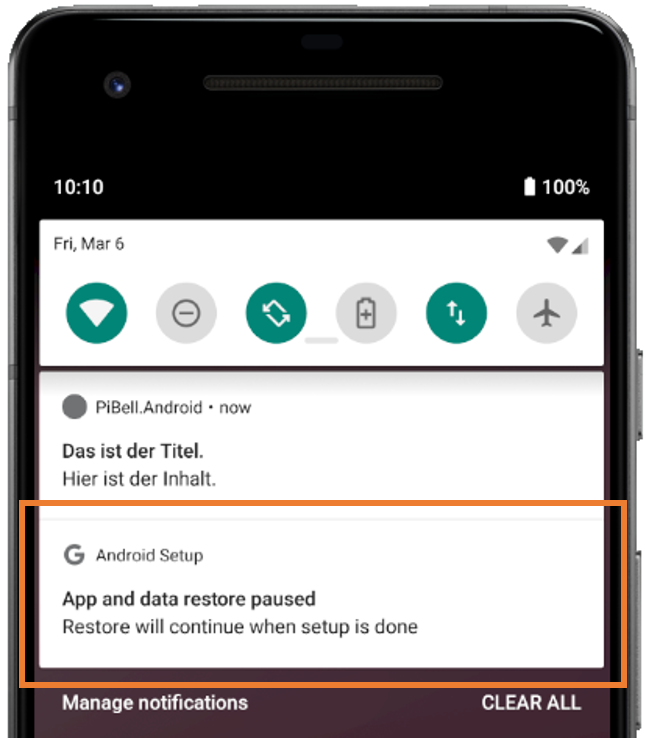
\includegraphics[width=.5\linewidth]{images/xamarin/LocalNotification.png}
    \caption{Lokale Benachrichtigung}
\end{figure}

Im Gegensatz dazu dient eine Push Notification dazu, den Benutzer über ein externes Ereignis auf einem anderen Gerät aufmerksam zu machen. Diese Art der Benachrichtigung findet meist Anwendung in der Katastrophenwarnung, um den Benutzer vor einer herannahenden Gefahr zu warnen.
Um den Benutzer also darüber zu informieren, dass jemand an der Haustür klingelt, wird eine Push Benachrichtigung verwendet, da das Anläut-Ereignis bei der Außenstation erfolgt.
\begin{figure}[H]
    \centering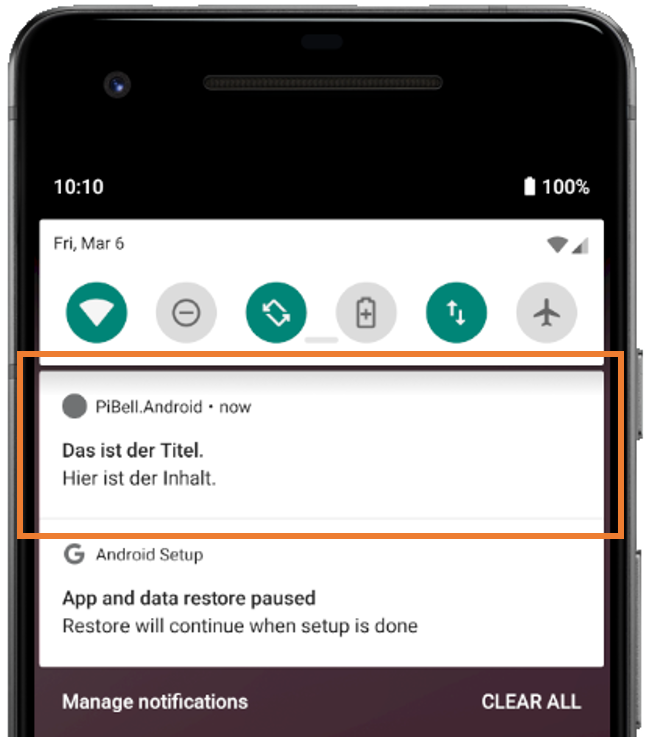
\includegraphics[width=.5\linewidth]{images/xamarin/PushNotification.png}
    \caption{Push-Benachrichtigung}
\end{figure}

\subsection{Funktionsweise}
Eine Push Notification wird immer von einem sogenannten Push Notification Service an alle Zielgeräte geschickt.
Dieser Service wird vom jeweiligen Betriebssystem-Hersteller bereitgestellt.
Im Fall der hier entwickelten App sind das Google und Apple, mit ihren Push Notification Services GCM und APNs.\par

Der Service ist dafür verantwortlich, die Benachrichtigung an alle registrierten Zielgeräte zu schicken.
Wenn das Zustellen nicht möglich ist, bricht der Service die Zustellung nach mehreren Versuchen für dieses Gerät ab.
Alle anderen Geräte erhalten die Benachrichtigung.
Daher ist es nicht sichergestellt, dass eine Push-Benachrichtigung bei jedem Gerät ankommt.\par

Zusätzlich zum Nachrichtentext können bei einer Push Notification zusätzliche Daten mitgeschickt werden. Diese können zum Beispiel die App über die genaue Benachrichtigungsursache informieren.

\section{AppCenter Push}
AppCenter Push hat in erster Linie die Funktion, den Zugriff auf die verschiedenen Push Notification Services zu vereinheitlichen und damit einfacher zu gestalten.
Microsoft AppCenter verwaltet alle Server-API-Schlüssel, Zielgerätelisten und ähnliche Einstellungen, um den Prozess des Benachrichtigung-Sendens zu vereinfachen.
AppCenter Push ist entweder über das Web-Interface unter \url{https://appcenter.ms/} oder über die AppCenter API erreichbar und verwendbar.\par

Die AppCenter Push \acs{sdk} abstrahiert den ganzen Prozess der Geräte-Registration, des Registrieren des Eingangs-Events und versteckt alles hinter einer einzelnen simplen Funktion \texttt{AppCenter.Start(„{App Secret}“, typeof(Push));}. Das App Secret ist der von AppCenter zugewiesene Schlüssel mit dem sichergestellt wird, dass das Gerät für das richtige AppCenter Projekt registriert wird.
Ohne diese \acs{sdk} müsste in der App viel mehr konfiguriert werden, was einen höheren Programmieraufwand und größere Fehlerrate darstellt. Außerdem würde das Rad neu erfunden werden.\par

In der entwickelten App wird die AppCenter-\acs{sdk}-Version 2.6.4 verwendet. Zu beachten ist, dass AppCenter Push nicht mehr weiterentwickelt und irgendwann dieses Jahr der Service abgeschaltet wird, wie es John Wargo in seinem Blog-Post am 3. Februar 2020 schrieb. Als Alternative wird von Microsoft der Azure-Notification-Hubs-Dienst angeboten. Bevor AppCenter Push endgültig terminiert wird, will Microsoft detaillierte Anleitungen zum Umstieg auf Azure bereitstellen.\par

\subsection{Konfiguration des \acs{sdk}}
Um AppCenter Push in der Applikation verwenden zu können, müssen mehrere NuGet-Pakete installiert werden.
Das AppCenter Paket beinhaltet alle Kernfunktionen wie AppCenter.Start(), das AppCenter-Push-Paket erweitert das Grundpaket um Push-bezogene Funktionen und Datentypen.
\begin{table}[H]
    \centering\begin{tabular}{|c|c|c|c|}
        \hline
        NuGet-Paket & PiBell & PiBell.Android & PiBell.iOS\\
        \hline
        AppCenter & Ja & Ja & Ja\\
        AppCenter Push & Ja & Ja & Ja\\
        \hline    
    \end{tabular}
    \caption{Installation NuGet-Pakete}
\end{table}